\documentclass[table,xcolor=dvipsnames]{beamer}\usepackage[]{graphicx}\usepackage[]{color}
%% maxwidth is the original width if it is less than linewidth
%% otherwise use linewidth (to make sure the graphics do not exceed the margin)
\makeatletter
\def\maxwidth{ %
  \ifdim\Gin@nat@width>\linewidth
    \linewidth
  \else
    \Gin@nat@width
  \fi
}
\makeatother

\definecolor{fgcolor}{rgb}{0.345, 0.345, 0.345}
\newcommand{\hlnum}[1]{\textcolor[rgb]{0.686,0.059,0.569}{#1}}%
\newcommand{\hlstr}[1]{\textcolor[rgb]{0.192,0.494,0.8}{#1}}%
\newcommand{\hlcom}[1]{\textcolor[rgb]{0.678,0.584,0.686}{\textit{#1}}}%
\newcommand{\hlopt}[1]{\textcolor[rgb]{0,0,0}{#1}}%
\newcommand{\hlstd}[1]{\textcolor[rgb]{0.345,0.345,0.345}{#1}}%
\newcommand{\hlkwa}[1]{\textcolor[rgb]{0.161,0.373,0.58}{\textbf{#1}}}%
\newcommand{\hlkwb}[1]{\textcolor[rgb]{0.69,0.353,0.396}{#1}}%
\newcommand{\hlkwc}[1]{\textcolor[rgb]{0.333,0.667,0.333}{#1}}%
\newcommand{\hlkwd}[1]{\textcolor[rgb]{0.737,0.353,0.396}{\textbf{#1}}}%

\usepackage{framed}
\makeatletter
\newenvironment{kframe}{%
 \def\at@end@of@kframe{}%
 \ifinner\ifhmode%
  \def\at@end@of@kframe{\end{minipage}}%
  \begin{minipage}{\columnwidth}%
 \fi\fi%
 \def\FrameCommand##1{\hskip\@totalleftmargin \hskip-\fboxsep
 \colorbox{shadecolor}{##1}\hskip-\fboxsep
     % There is no \\@totalrightmargin, so:
     \hskip-\linewidth \hskip-\@totalleftmargin \hskip\columnwidth}%
 \MakeFramed {\advance\hsize-\width
   \@totalleftmargin\z@ \linewidth\hsize
   \@setminipage}}%
 {\par\unskip\endMakeFramed%
 \at@end@of@kframe}
\makeatother

\definecolor{shadecolor}{rgb}{.97, .97, .97}
\definecolor{messagecolor}{rgb}{0, 0, 0}
\definecolor{warningcolor}{rgb}{1, 0, 1}
\definecolor{errorcolor}{rgb}{1, 0, 0}
\newenvironment{knitrout}{}{} % an empty environment to be redefined in TeX

\usepackage{alltt}


\usepackage{xcolor}
\usepackage{url}
\usepackage{amsmath}
\usepackage{amsthm}
\usepackage{amssymb}
\usepackage{graphicx}
\usepackage{tikz}
\usetikzlibrary{shapes,arrows}
\usepackage{float}
\usepackage{verbatim}
\usepackage{hyperref}

\usepackage{lmodern,tabularx,ragged2e,booktabs}
\newcolumntype{Y}{>{\arraybackslash\RaggedRight}X}
\newcolumntype{P}[1]{>{\arraybackslash\RaggedRight}p{#1}}


\usetheme{Szeged}
\usecolortheme[named=RoyalBlue]{structure}


% Personal Data


\title[High Resolution Identification of Protein-DNA Binding Events]{High Resolution Identification of Protein-DNA Binding Events
  and Quality Control for ChIP-exo data}

\author{Rene Welch\\Preliminary Examination}

\institute[UW-STAT]{Department of Statistics\\University of Wisconsin - Madison}


\date{December 1st, 2015}

\newcommand{\sig}{\sigma^{70}}
\IfFileExists{upquote.sty}{\usepackage{upquote}}{}
\begin{document}


\begin{frame}
  \maketitle
\end{frame}

\begin{frame}
\frametitle{Outline}
  \tableofcontents
\end{frame}

\section{ChIP-exo procedure}

\begin{frame}
\frametitle{ChIP-exo procedure}
  \begin{figure}[H]
    \centering
\includegraphics{../figs/diagrams/ChIPexo_diagram1.png}
\includegraphics{../figs/diagrams/ChIPexo_diagram2.png}\\
\includegraphics{../figs/diagrams/ChIPexo_diagram3.png}
    \caption{ChIP-exo procedure, the diagram is from Furey, 2012 \cite{chipbeyond}}
    \label{fig:exo_diagram}
  \end{figure}
\end{frame}

\section{ChIP-Seq QC measures}
\begin{frame}
  \frametitle{ChIP-Seq QC measures}

\only<1>{
\setlength\tabcolsep{3pt}  % default value: 6pt
\scriptsize  %%  command to change the font size
\rowcolors{1}{}{RoyalBlue!20} %-- this indicates the change in odd and pair rows
\begin{tabularx}{\textwidth}{ @{} c|   Y @{}}
  \toprule
  \textbf{QC measure} & \textbf{Definition} \\
  \midrule
  Nr. reads & Self-explanatory. The higher the better...  \\
  PCR bottleneck Coeff. &  Ratio of number of pos. to which EXACTLY one read maps and number  of pos. to which AT LEAST one read maps \\
  Standarized Std. Dev. &  Normalized Std. Deviation of the sequencing coverage \\
  Strand Cross-Corr. &  $  y(\delta) = \sum_c w_c r\left[ n_c^+ \left(x + \frac{\delta}{2}
    \right), n_c^- \left( x- \frac{\delta}{2} \right)\right]$ \\
  Normalized SCC &  Ratio of max value of SCC and min value of SCC$^*$  \\
  \bottomrule
\end{tabularx}
}

\only<1>{
where $n_c^S$ is the coverage for chromosome $c$ and strand $S$. $r$ is
the Pearson correlation and $w_c$ is the proportion of reads in the
experiment for chromosome $c$
}

\only<2>{
\setlength\tabcolsep{3pt}  % default value: 6pt
\scriptsize  %%  command to change the font size
% \rowcolor{RoyalBlue!20} %-- this indicates the change in odd and pair rows
\begin{tabularx}{\textwidth}{ @{} c|c|c|c|c|c|c| Y @{}}
  \toprule
IP & Organism  &Condition & Rep. & Nr. reads & PBC & SSD &  NSC  \\
\midrule
\rowcolor{RoyalBlue!20}$\sig$ & E.Coli & Rif-0min & 1 & 960,256 & 0.2823 & 0.0361 &  10.29 \\
\hline
\rowcolor{RoyalBlue!20}$\sig$ &  E.Coli & Rif-0min & 2 & 2,247,295 & 0.2656 & 0.1091  &  25.08  \\
\hline
\rowcolor{RoyalBlue!20}$\sig$ &  E.Coli & Rif-20min & 1 & 1,940,387 & 0.2698 & 0.0820  & 17.69  \\
\hline
\rowcolor{RoyalBlue!20}$\sig$ &  E.Coli & Rif-20min & 2 & 4,229,574 & 0.2153 & 0.1647  &  14.11 \\
\hline
\rowcolor{Red!20}FoxA1 &  Mouse &  - & 1 & 22,210,461 & 0.6562 & 9.12 $\times 10^{-5}$ & 21.452 \\
\hline
\rowcolor{Red!20}FoxA1 &  Mouse &  - & 2 & 22,307,557 & 0.7996 & 7.94 $\times 10^{-5}$ & 60.661 \\
\hline
\rowcolor{Red!20}FoxA1 &  Mouse &  - & 3 & 22,421,729 & 0.1068 & 1.31 $\times 10^{-4}$ & 72.312 \\
\hline
\rowcolor{Green!20}ER & Human & - & 1 & 9,289,835 & 0.8082 & 3.64 $\times 10^{-5}$ & 19.843 \\
\hline
\rowcolor{Green!20}ER & Human & - & 2 & 11,041,833 & 0.8024 & 4.6 $\times 10^{-5}$ & 21.422 \\
\hline
\rowcolor{Green!20}ER & Human & - & 3 & 12,464,836 & 0.8203 & 4.89 $\times 10^{-5}$ & 19.699 \\
\hline
\rowcolor{Yellow!20}CTCF & Human & - & 1 &   48,478,450 & 0.4579 & 1.29 $\times 10^{-4}$ & 15.977 \\
\bottomrule
\end{tabularx}  
}

\end{frame}


\section{Comparison of ChIP-exo and ChIP-seq}

\begin{frame}[plain]
  \frametitle{Comparison of ChIP-exo and ChIP-seq - SCC}  
\begin{figure}[H]
  \centering  
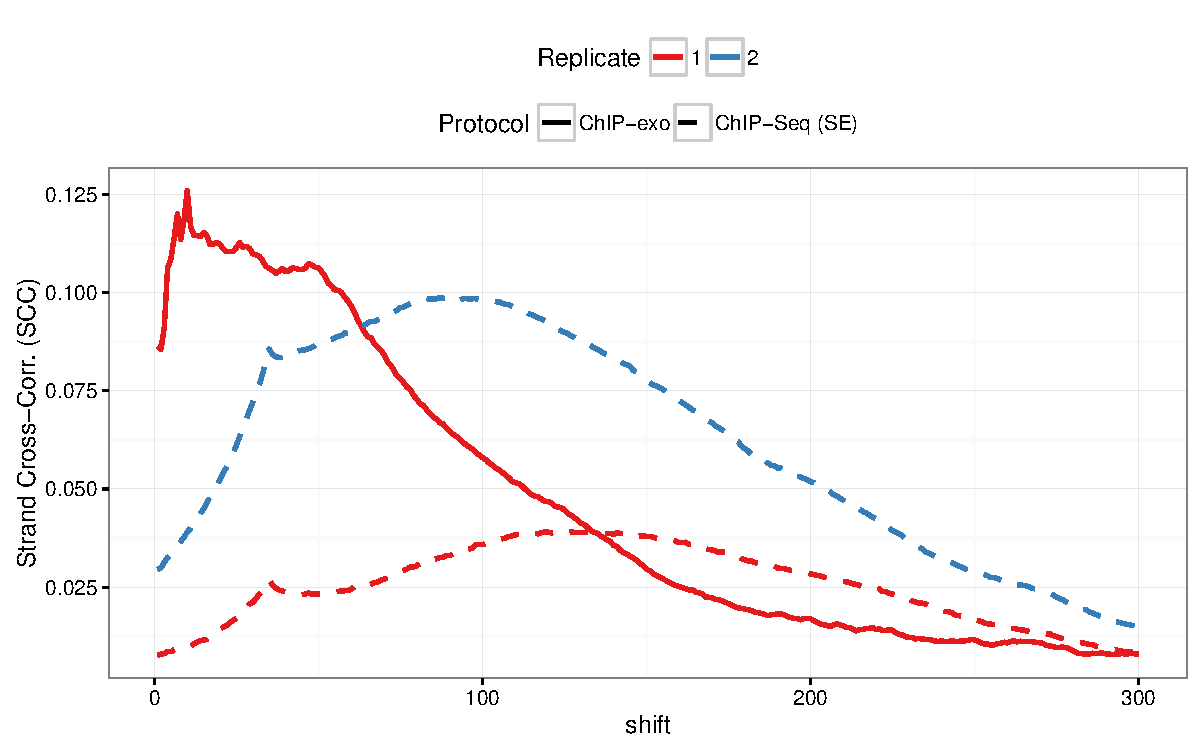
\includegraphics[width = .7\textwidth]{../figs/for_paper/scc_ctcf.pdf}
\caption{SCC for CTCF factor in HeLa cell line for ChIP-exo and
  SET-ChIP-Seq }
  \label{fig:scc}
\end{figure}

\begin{itemize}
\item There is a \emph{``phantom peak''} at read length.
\item In ChIP-Seq SCC is maximized at the unobserved fragment length.
\item In ChIP-exo, the \emph{``phantom peak''} and the frag. length
  summit are confounded.
\end{itemize}

\end{frame}


\begin{frame}
  \frametitle{Comparison of ChIP-exo and ChIP-Seq}

\begin{figure}[H]
  \centering
  \includegraphics[width = .5\textwidth,page = 3 ]{../figs/for_paper/ChIPseqPET_ChIPexo_tagCount_comparison.pdf}
  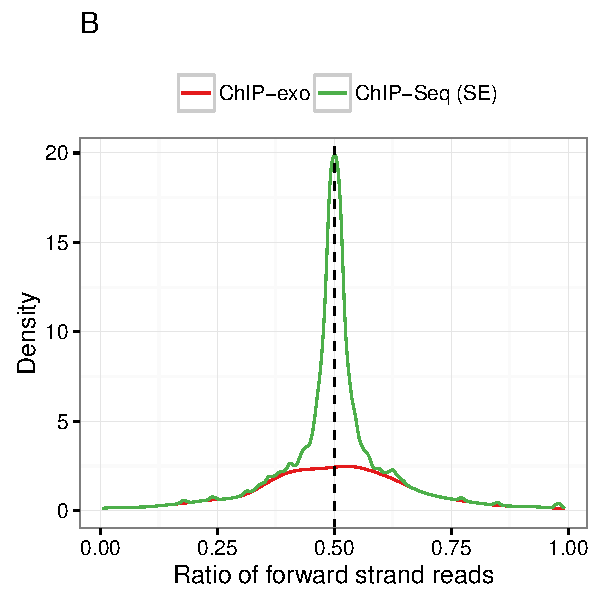
\includegraphics[width = .5\textwidth]{../figs/for_paper/forward_strand_ratio_comp_old.pdf}
\end{figure}

\begin{itemize}
\item
\item 
\end{itemize}

% \only<2>{
% \begin{figure}[H]
% \centering
% 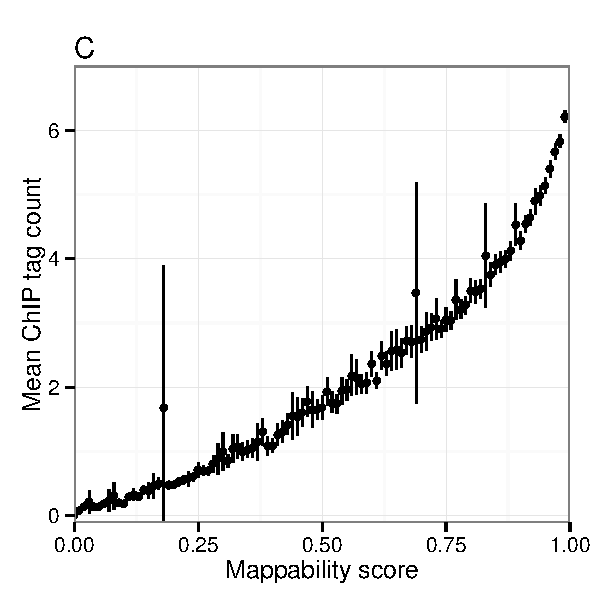
\includegraphics[width = .46\textwidth,page = 1]{../figs/for_paper/eukaryotic_bias_CTCF.pdf}
%   \includegraphics[width = .46\textwidth,page = 2]{../figs/for_paper/eukaryotic_bias_CTCF.pdf}
% \end{figure}
% }
\end{frame}


\begin{frame}[t]
\frametitle{Software}  
\begin{itemize}
\item \textbf{dPeak}: We updated the initialization strategy. The
  latest version is currently available from
  \url{http://dongjunchung.github.io/dpeak/}.
\item \textbf{ChIPexoQual}: This package contains the QC pipeline for
  ChIP-exo. The last version is available in
  \url{https://github.com/welch16/ChIPexoQual}.
\item \textbf{Segvis}: The goal of this package is to visualize
  genomic regions by using aligned reads. The latest version is
  available in \url{https://github.com/keleslab/Segvis}.
\item \textbf{ChIPUtils}: This package attempts to gather the most
  commonly used ChIP-Seq QC.The latest available version is in
  \url{https://github.com/welch16/ChIPUtils}.
\end{itemize}

\end{frame}

\begin{frame}
  \frametitle{References}

{\tiny

\nocite{exo1}
\nocite{dpeak}

\bibliographystyle{plain} % Style BST file (bmc-mathphys, vancouver, spbasic)
\bibliography{chip_exo_paper}

}

\end{frame}

\end{document}
